\documentclass[letterpaper,10pt,twocolumn,titlepage]{article}

\usepackage{graphicx}                                        
\usepackage{amssymb}                                         
\usepackage{amsmath}                                         
\usepackage{amsthm}                                          

\usepackage{alltt}                                           
\usepackage{float}
\usepackage{color}
\usepackage{url}

\usepackage{balance}
\usepackage[TABBOTCAP, tight]{subfigure}
\usepackage{enumitem}
\usepackage{pstricks, pst-node}

\usepackage{fancyhdr}
\pagestyle{fancy}
\usepackage{geometry}
\geometry{textheight=8.5in, textwidth=6in}

%random comment

\newcommand{\cred}[1]{{\color{red}#1}}
\newcommand{\cblue}[1]{{\color{blue}#1}}

\usepackage{hyperref}
\usepackage{geometry}

\def\name{Jonah Brooks}

%% The following metadata will show up in the PDF properties
\hypersetup{
  colorlinks = true,
  urlcolor = black,
  pdfauthor = {\name},
  pdfkeywords = {cs311 ``operating systems'' process exec pipe sort},
  pdftitle = {CS 311 Project 2: UNIX Process control},
  pdfsubject = {CS 311 Project 2},
  pdfpagemode = UseNone
}

\begin{document}

\fancyhead[R]{Jonah Brooks \linebreak CS311 HW2 \linebreak 02-07-2012}


\section{UNIX Process Control}

This is the write-up for assignment 2 of CS311. 
In this assignment, I created a program (h2.cpp) that accepts input from stdin,
parses that input into case insensitive words delimeted by punctuation, sorts those
words using a number of sort processes, then collects the sorted output and merges it 
together into one single list of unique words, returning this list via stdout.
I also timed my code running 10\textsuperscript{n} words from the bible, 
and from random lipsum text. The graphs of the time taken for each test for 
values of n from 1 to 6 is on page 2 of this document.
 
\section{Design Decisions}

I chose to implement my code using a number of functions: 
parser, sorter, suppressor, normalize, and index\_of\_smallest.
Each of these functions is designed for a single purpose; parser,
sorter, and suppressor each hold the sections of code that should
be run by the process of its titular type. This structure made it
much easier for me to wrap my head around the parallel nature of
this project, since I only needed to call a single function once
I determined which process was running after the fork. This also
allowed me to write my code in each function knowing that no other
process type could access it.

The other two functions are used for formatting and handling the
input and output, respectively. normalize takes a word, forces every
character to lower case, and removes all non-essential punctuation, 
leaving apostrophes and hyphens, but treating all other special 
characters as token delimeters. I chose these punctuations since
I wanted words such as "that's" to count differently than "that,"
and because I wanted to count "compound-words" as one word. I left
out all other punctuation because I did not want to count line of code 
such as "while(a=b+c)" to count as only one word. This has the unfortunate 
issue of breaking words on accented characters and non-standard apostrophes, 
but I think it works well, and efficently, for most documents an English 
speaker would want to parsing.

index\_of\_smallest was used to allow me to more easily merge
the sorted lists back together into one single list. I chose to
implement a very modified merge-sort algorithm for this purpose,
in which I would take the smallest word from all visible words 
(effectively the ends of the pipes), print it to stdout (unless it
is the same as the last printed word), then refresh the list of 
visible words before I repeat. This way I needed only one array that
holds one word from each pipe, since I'm merging them into the output
stream rather than a new array.

\section{Commit Log}

\begin{tabular}{ | p{3cm} | p{5.5cm} | }
	\hline
	Commit Time & Commit Message \\ \hline
	\input{git_log_table}
\end{tabular}

\vfill\break

\fancyhead{}

\begin{figure}[h]
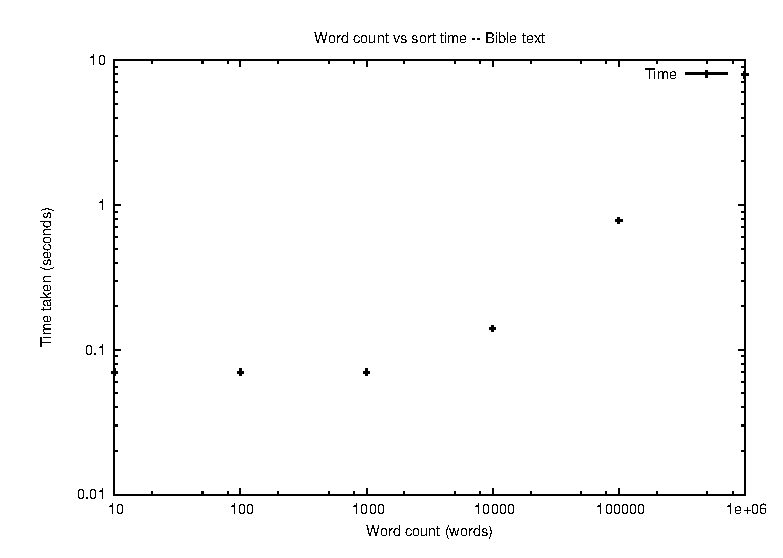
\includegraphics{bible_log.eps}
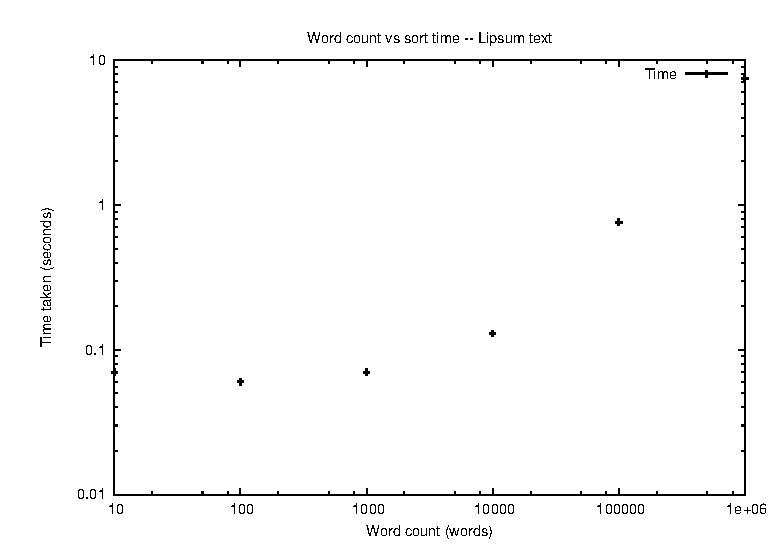
\includegraphics{lipsum_log.eps}  
\end{figure}

\end{document}
















